\section{Zusammenwirken mehrerer Systeme}
\subsection{Regelkreis}
	\begin{mdframed}[style=exercise, frametitle=Wichtige Begriffe]
		\begin{itemize}[leftmargin=*]
			\item Führungsgröße: w(t)
			\item Störgröße: z(t)
			\item Regelgröße: x(t)
			\item Regeldifferenz: e(t) = w(t) - x(t)
			\item Maximale Überschwingweite: maximale Regelabweichung nach dem erstmaligen Erreichen des Sollwertes
			\item Anregelzeit: Zeit zum erstmaligen Erreichen des Sollwertes
			\item Ausregelzeit: Zeit zum dauerhaften Erreichen des Sollwertes im Toleranzband
		\end{itemize}
	\end{mdframed}

	\begin{mdframed}[style=exercise,frametitle=Anforderungen:]
		\begin{itemize}[leftmargin=*]
			\item Stabilität: Regelkreis muss stabiles Verhalten zeigen (gilt
				auch für instabile Systeme)
			\item Gutes Führungsverhalten: Die Differenz zw. Sollwert w(t) und
				Istwert x(t) muss schnell klein werden.
			\item Gutes Störverhalten: Einfluss von Störgrößen soll vermindert
				werden.
		\end{itemize}
	\end{mdframed}

	Grundstruktur des einschleifigen Regelkreises:

	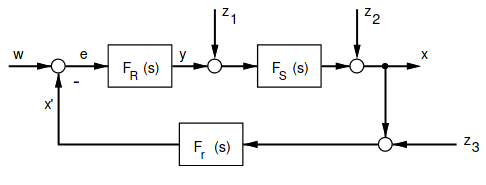
\includegraphics[width=0.8\columnwidth]{Figures/zusammenwirkenMehrererSysteme/einschleifigerRegelkreis.png}

	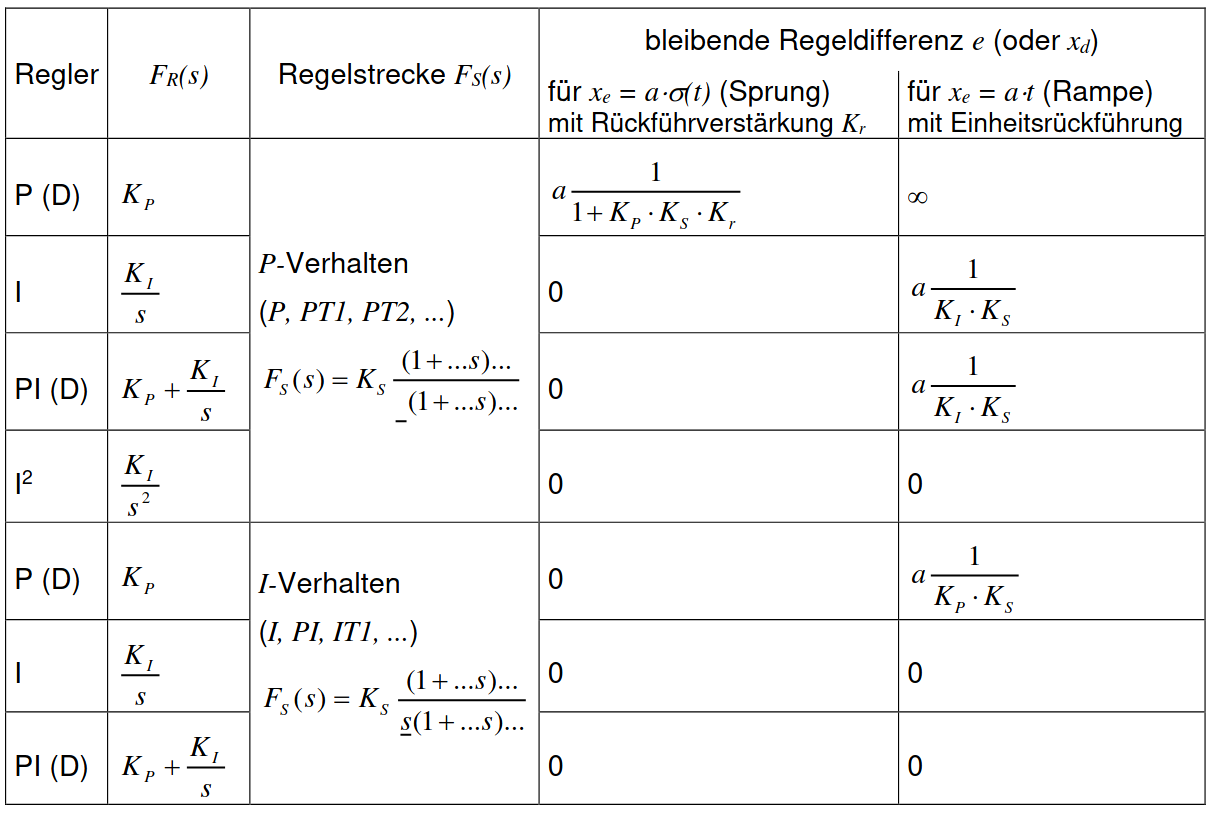
\includegraphics[width=\columnwidth]{Figures/zusammenwirkenMehrererSysteme/Reglerauswahl.png}

	Grundsätzliche Eigenschaften der Kreisstruktur: 

	\begin{figure}[H]
			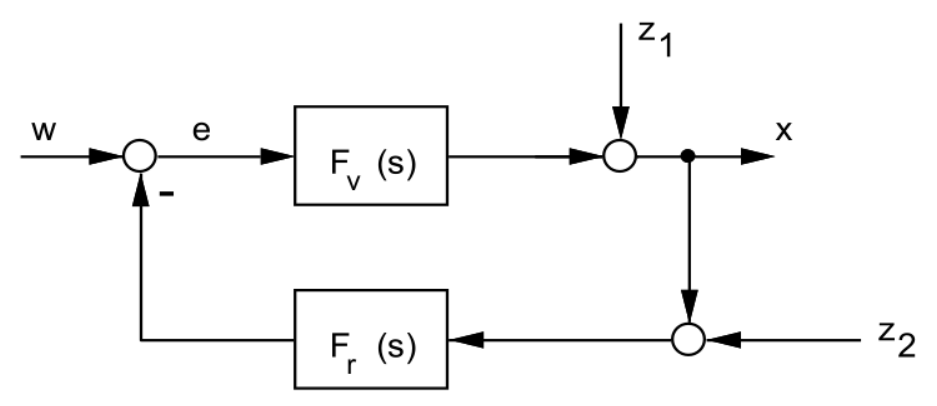
\includegraphics[width=0.8\columnwidth]{Figures/zusammenwirkenMehrererSysteme/Kreisstruktur.png}
	\end{figure}
	\begin{align*}
		X &= \frac{F_V}{1+F_V \cdot F_r}\cdot W + \frac{1}{1 + F_V \cdot F_r} \cdot Z_1 + \frac{- F_V \cdot F_r}{1 + F_V \cdot F_r} \cdot Z_2 \\
		F_w &= \frac{F_V}{1+F_V \cdot F_r} \text{ (Führungsübertragungsfunktion)}\\
		F_{z1} &= \frac{1}{1 + F_V \cdot F_r} \text{ (Störübertragungsfunktion 1)}\\
		F_{z2} &= \frac{- F_V \cdot F_r}{1 + F_V \cdot F_r} \text{ (Störübertragungsfunktion 2)}
	\end{align*}

\subsection{Wurzelortskurven (WOK)-Verfahren}
	\begin{mdframed}[style=exercise]
		Reglerfunktion $F_R$ in Reglerverstärkung und Reglerdynamik aufspalten:
		$F_R =K \cdot F_R ' $
	\end{mdframed}

	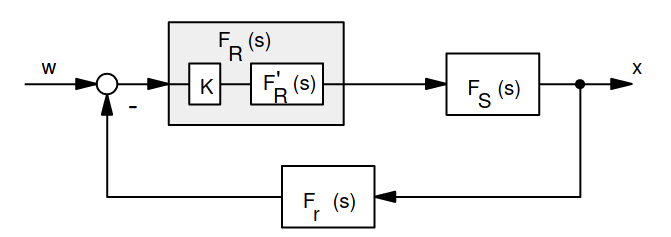
\includegraphics[width=0.94\columnwidth]{Figures/zusammenwirkenMehrererSysteme/WOKkreis.png}\\
	\(
		\Rightarrow F_w (s)= \dfrac {F_R \cdot F_S} {1+F_R \cdot F_S \cdot F_r} = \dfrac {F_R \cdot F_S} {1+F_o}
	\)

	\begin{align*}
		F_o (s) & = F_R (s) \cdot F_S (s) \cdot F_r (s) \\
		& =K \cdot F_R '(s) \cdot F_S (s) \cdot F_r (s) \\
		& =K \cdot Q \cdot \frac{\prod_{\mu=1}^{m}\left(s-s_{\color{red}{N0\mu}}\right)}{\prod_{\vartheta=1}^{n}\left(s-s_{\color{red}{P0\vartheta}}\right)}
	\end{align*}

	Für eine Polstelle muss der Nenner von $F_w (s)$ Null werden:
	\begin{align*}
		\dfrac{F_R (s) \cdot F_S (s)}{1+F_o (s)} \Rightarrow 1+F_o (s) \stackrel{!}{=}0 \\
		\Rightarrow \frac{\prod_{\vartheta=1}^{n}\left(s-s_{\color{red}{P0\vartheta}}\right)}{\prod_{\mu=1}^{m}\left(s-s_{\color{red}{N0\mu}}\right)} = -K \cdot Q
	\end{align*}

	Diese Gleichung kann in Betrag und Phase aufgeteilt werden:
	\begin{align*}
		& \frac{\prod_{\vartheta=1}^{n}\left|s-s_{\color{red}{P0\vartheta}}\right|}{\prod_{\mu=1}^{m}\left|s-s_{\color{red}{N0\mu}}\right|} = |K \cdot Q|
	\end{align*}
	Falls keine Nullstellen vorliegen, ist der Nenner zu 1 zu wählen.
	\begin{align*}
		& \sum_{\vartheta=1}^{n} \angle\left(s-s_{\color{red}{P0\vartheta}}\right) - \sum_{\mu=1}^{m} \angle\left(s-s_{\color{red}{N0\mu}}\right) = \angle\left(-K \cdot Q\right) = \pm r \cdot 180^\circ \\
		& \qquad r = 1,3,5,\ldots \text{ für }K \cdot Q > 0 \\
		& \qquad r = 0,2,4,\ldots \text{ für }K \cdot Q < 0
	\end{align*}

	Aus der Phasenbeziehung lässt sich der Verlauf der WOK bestimmen.\\
	{\footnotesize Wenn Betragsbedingung erfüllt \textrightarrow Punkt ist Teil der WOK}
	\\
	\\
	Die Betragsbeziehung gestattet es, jedem Punkt der WOK den entsprechenden \(K\)-Wert zuzuordnen. \\
	{\footnotesize 
		entsprechenden \(s\)-Wert einsetzen \\
		\(K_{Krit}\) durch einsetzen von \(s_{Krit}\) (Punkt an dem WOK durch Imaginär-Achse geht)\\
		Stabilität für \(K > K_{Krit}\) oder \(K < K_{Krit}\) aus der WOK ablesen.
	}

	\begin{mdframed}[style=exercise, frametitle=Konstruktion der WOK]
		\begin{enumerate}[leftmargin=*]
			\item Alle n Äste der WOK beginnen mit K=0 in den n Polen $s_{Po_v}$ des offenen Regelkreises.
			\item m Äste der WOK enden für K $\rightarrow \pm \infty$ in den \(m\) endlichen Nullstellen $s_{No_v}$ des offenen Regelkreises 
			\item \(n - m\) Äste der WOK enden für K $\rightarrow \pm \infty$ im Unendlichen. \(n - m\) ist der Polüberschuss.
			\item Die n-m ins Unendliche strebende Äste der WOK haben Asymptoten, die\\
				a) im Wurzelschwerpunkt
				\begin{align*}
					s_{w}=\frac{\sum_{v=1}^{n} s_{pov}-\sum_{u=1}^{m} s_{_{Nop}}}{n-m}
				\end{align*}
				beginnen und die dabei\\
				b) mit der reellen Achse die Winkel
				\begin{align*}
					\varphi_{k} &= \frac{(2 k-1) \cdot 180^{\circ}}{n-m} \text{ für } KQ > 0 \\
					\text{bzw. } \varphi_{k} &= \frac{(2 k-2) \cdot 180^{\circ}}{n-m} \text{ für } KQ < 0 \\
					\text{mit } k &= 1,2,3,\ldots,n-m
				\end{align*}
				einschließen.
			\item Die Punkte der WOk liegen entweder auf der reelen Achse, oder symmetrisch zur reelen Achse
			\item Ein Punkt s auf der reellen Achse ist dann ein Punkt der WOK, wenn sich bei KQ > 0 (KQ<0)
				rechts von ihm eine ungerade (gerade) Anzahl von Polen $s_{Po_v}$ und (+) Nullstellen $s_{No_v}$ befindet.
		\end{enumerate}

		Achtung: WOK ist nicht anwendbar, wenn es sich um nicht rationale
		Übertragungsfunktionen handelt.\\ (z.B. Regelkreis mit Totzeitverhalten!)
	\end{mdframed}

\subsection{Nyquist Kriterium}
	\begin{center}
		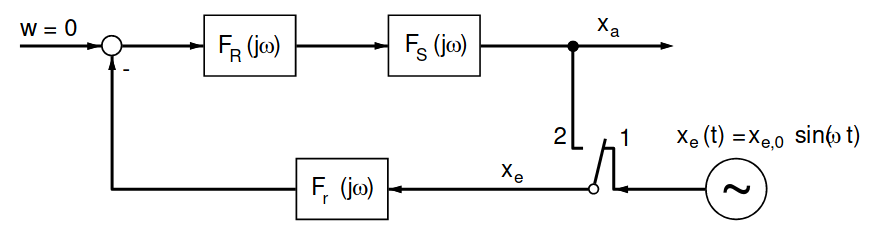
\includegraphics[width=.45\textwidth]{Figures/zusammenwirkenMehrererSysteme/Nyquist.png}
	\end{center}
	Frequenzgangfunktion des offenen Regelkreises:
	\begin{align*}
		F_o (j\omega) = F_r (j\omega) \cdot F_R (j\omega) \cdot F_S (j\omega)
	\end{align*}

	Ausgangssignal:
	\begin{align*}
		x_a(t) &= -F_o (j\omega) \cdot x_e (t)
	\end{align*}

	Regler und seine Parameter werden so gewählt,\\ dass $\omega = \omega_{krit}$ gilt:
	\begin{align*}
		F_o (j\omega_{krit})=-1 \texttt{ (Schwingbedingung)}
	\end{align*}

	\begin{mdframed}[style=exercise]
		Die Schwingbedingung ist erfüllt, wenn die Ortskurve von $F_o (j\omega)$
		durch den kritischen Punkt ($P_{krit} = -1+j0$) der komplexen $F_o$-Ebene
		geht.

		An diesem Punkt kann man $\omega_{krit}$ ablesen (damit kann der Regelkreis
		Dauerschwingungen ausführen).

		Für größere Verstärkung ist das System instabil, für kleinere stabil.
	\end{mdframed}

	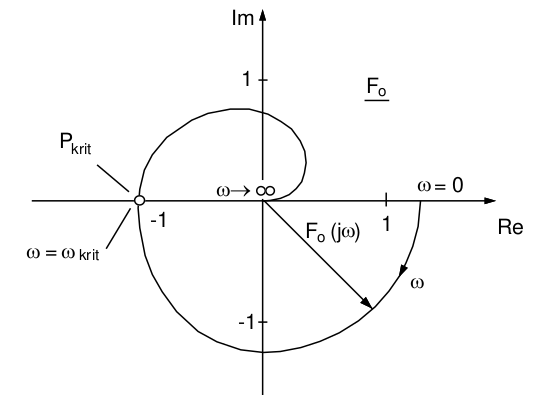
\includegraphics[width=0.94\columnwidth]{Figures/zusammenwirkenMehrererSysteme/Nyquistwkrit.png}

	\begin{mdframed}[style=exercise, frametitle=vereinfachtes Nyquist-Kriterium:]
		Falls F(s) des offenen Kreises keine Pole in der rechten Halbebene hat und
		nur max. 2 im Ursprung der s-Ebene, ist der Regelkreis stabil, wenn: \\
		Beim Durchlaufen der Ortskurve von $F_o (j\omega)$ für $\omega$ von 0 bis $\infty$ der
		kritische Punkt \(F_o(j \omega_{krit} = -1 + 0j)\) auf der linken Seite der Ortskurve liegt.
	\end{mdframed}

	Zur Auswertung des Nyquist-Kriteriums im Bode Diagramm, spaltet man die Ortskurve nach Betrag
	A = $|F_0 (jw)|$ und Phase $\varphi$ = $arg(F_0(jw))$

	\begin{figure}[H]
		\centering
		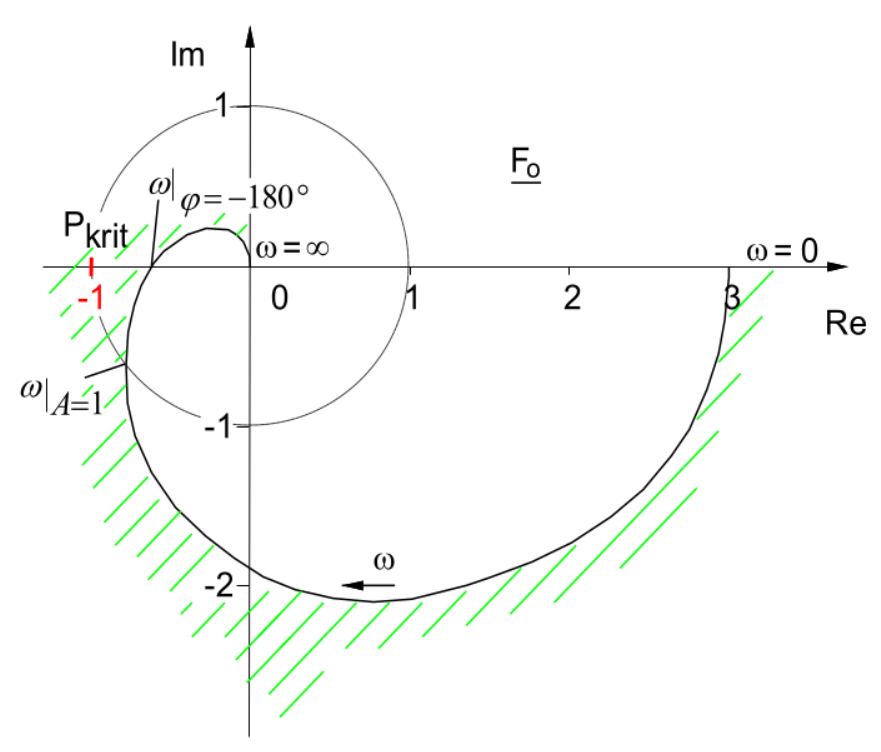
\includegraphics[width=0.6\columnwidth]{Figures/zusammenwirkenMehrererSysteme/Nyquist_Bode_1.png}
		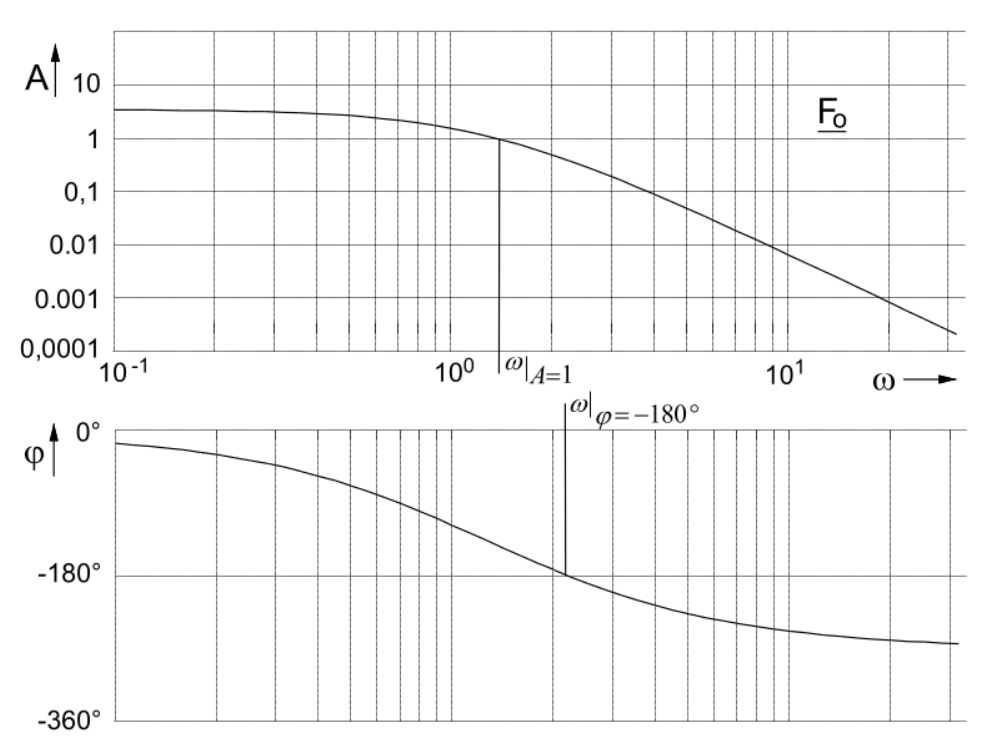
\includegraphics[width=\columnwidth]{Figures/zusammenwirkenMehrererSysteme/Nyquist_Bode_2.png}
	\end{figure}

	\begin{center}
		\textbf{Stabilität für: } \(\left. \omega \right|_{A=1} < \left. \omega \right|_{\varphi = -180^\circ}\)
	\end{center}


	\textbf{Falls die vereinfachte Bedingung nicht funktioniert, wird die allgemeine Formulierung verwendet:}

	\begin{mdframed}[style=exercise, frametitle=Allgemeines Nyquist-Kriterium:]
		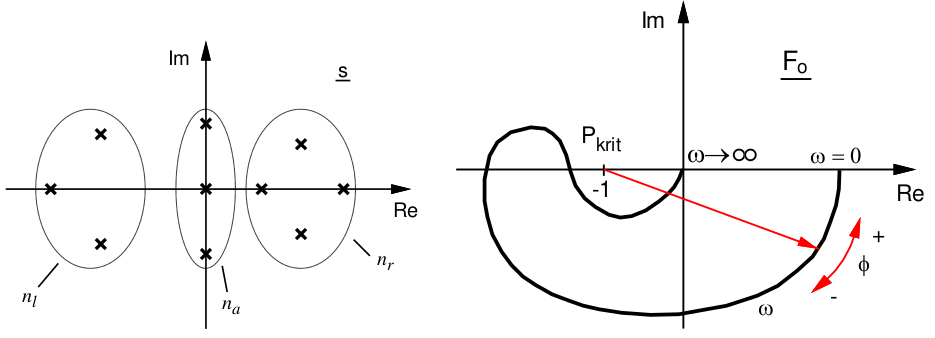
\includegraphics[width=0.94\columnwidth]{Figures/zusammenwirkenMehrererSysteme/Allgemein_Nyquist.png}

		Der geschlossene Regelkreis ist stabil, wenn der Fahrstrahl von $P_{krit}$ = -1 +j0
		zu $F_0 (jw)$ für wachsendes $\omega$ von +0 bis +$\infty$ eine Winkeländerung
		\begin{align*}
			^{\omega=+\infty}_{\omega=+0} \Delta \phi _{soll} = n_r \cdot 180^\circ +n_a \cdot 90^\circ
		\end{align*}
		erfährt.\\
		$n_r$: Anzahl der Pole rechts der imaginären Achse\\
		$n_a$: Anzahl der Pole auf der imaginären Achse
	\end{mdframed}


\begin{minipage}{\columnwidth}
	\subsection{Reglerauslegung im Bode Diagramm}
		Folgende Anforderungen für einen Regler: 
		\begin{mdframed}[style=exercise]
			\begin{itemize}[leftmargin=*]
				\item kleine bleibende Regeldifferenz: \(A(\omega) \gg 1 \text{ bei } \\ \omega \ll \left.\omega\right|_{A=1} \)
				\item Stabilität: \( \left.\varphi\right|_{A=1} > -180^\circ\)
				\item Phasenrand: \(\varphi_R = \left.\varphi\right|_{A=1} + 180^\circ\)\\
					befriedigendes Störverhalten: \(\varphi_R \ge 30^\circ\) \\
					gutes Führungsverhalten (überschwindungsarm): \(\varphi_R \approx 60^\circ\) \\
					gutes Führungsverhalten (überschwingungsfrei): \(\varphi_R \ge 80^\circ\) 
				\item Unterdrückung von Störgrößen: \(A(\omega) \ll 1 \text{ bei } \\ \omega \gg \left.\omega\right|_{A=1} \)
			\end{itemize}
		\end{mdframed}
\end{minipage}

		

\subsection{Einstellregeln}
	\subsubsection{Zeigler/Nichols}
		Zur Bestimmung der Reglerparameter wird der Regelkreis zunächst mit einem reinen P-Regler betrieben. 
		Dabei wird die Reglerverstärkung \(K_P\) so lange erhöht, bis der Regelkreis Dauerschwingungen ausführt.
		Diese kritische Verstärkung \(K_{P,krit}\) und die Periodendauer \(T_{krit}\) der Schwingung werden notiert.
		\begin{figure}[H]
			\centering
			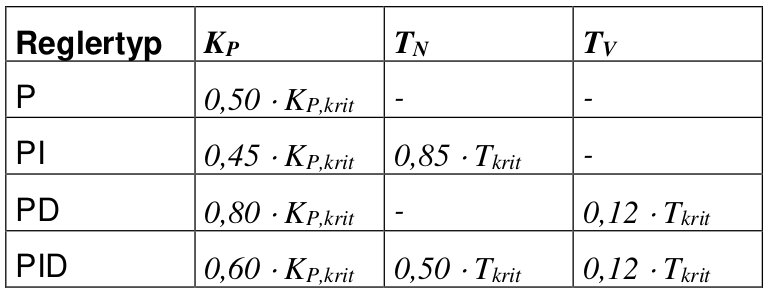
\includegraphics[width=0.9\columnwidth]{Figures/zusammenwirkenMehrererSysteme/ZieglerNich.png}
		\end{figure}		
		Ein Nachteil dieses Verfahrens ist, dass das System bis zum Schwingen gebracht werden muss (Stabilitätsgrenze), was nicht bei allen Regelstrecken zulässig ist (Zerstörung).

	\subsubsection{Betragsoptimum}
		Anwendbar für Systeme mit Streckenverhalten \(PT_n\) mit einer „dominierenden“ (großen) und mehreren kleinen Zeitkonstanten (möglichst reelle Pole):\\
		{ \footnotesize Berechnung inklusive des Rückführteils}
		\begin{align*}
			&T_1 = T_d \gg T_2, T_3, \ldots, T_n \qquad T_\Sigma = \sum T_2, T_3, \ldots, T_n\\
			&\text{Streckenverstärkung: } K_S = K_1 \cdot K_2 \cdot \ldots \cdot K_n \\
			&\Rightarrow \text{PI-Regler: } F_{PI} = K_R \cdot \left(1 + \frac{1}{T_N \cdot s}\right)\\
			&\text{mit } T_N = T_d \quad \text{;} \quad K_R = \frac{T_d}{2 \cdot K_S \cdot T_\Sigma}
		\end{align*}

	\subsubsection{Symmetrisches Optimum}
		Anwendbar für Systeme mit Streckenverhalten \(IT_n\) (reelle Pole notwendig):\\
		{ \footnotesize Berechnung inklusive des Rückführteils}
		\begin{align*}
			&T_\Sigma = \sum T_1, T_2, \ldots, T_n \\
			&\text{Streckenverstärkung: }K_S = K_1 \cdot K_2 \cdot \ldots \cdot K_n \\
			&\Rightarrow \text{PI-Regler} (\varphi_R \approx 40^\circ): \\
			&F_{PI} = K_R \cdot \left(1 + \frac{1}{T_N \cdot s}\right) \\
			&\text{mit } T_N = 4 \cdot T_\Sigma \quad K_R = \frac{1}{2 \cdot K_S \cdot T_\Sigma}
		\end{align*}
		


\subsection{Maßnahmen zur Verbesserung des Regelverhaltens}
	\raggedright
	\begin{mdframed}[style=exercise, frametitle=Störgrößenaufschaltung:]
		Falls Angriffsort einer Störgröße bekannt und Störgröße messbar,kann man wie im Bild kompensieren.\\
		Vorteil: einfacher Regler Entwurf, deutlich schnellere Ausregelung.
	\end{mdframed}
	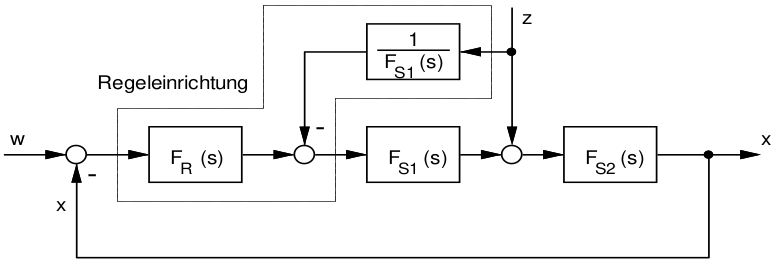
\includegraphics[width=0.9\columnwidth]{Figures/zusammenwirkenMehrererSysteme/Stoergoesenschaltung.png}

	\begin{mdframed}[style=exercise, frametitle=Vorsteuerung:]
		Geeignet, falls kein Kompromiss für gutes Stör und Folgeverhalten.\\
		Regler ist auf gutes Störverhalten ausgelegt. Mit $F_{Rv}$ wird ein schnelles Folgen
		auf Führungssignale w(t) erreicht.
	\end{mdframed}
	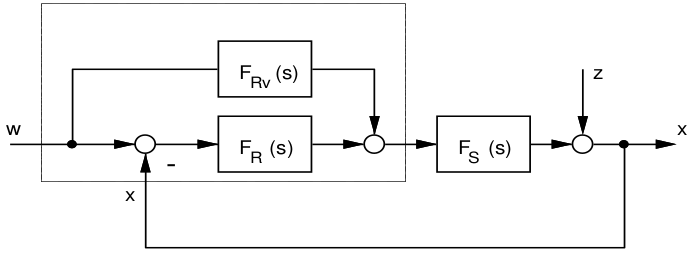
\includegraphics[width=0.9\columnwidth]{Figures/zusammenwirkenMehrererSysteme/Vorsteuerung.png}

	\begin{mdframed}[style=exercise, frametitle=Kaskadenregelung:]
		Ineinander geschachtelte Regelkreise (innere Regelkreise „schneller“). „Innere“
		Störungen können bereits innen ausgeregelt werden. Können von Innen nach Außen in Betrieb genommen werden.

		In WOK: \(K\) für innere Kreise muss festgelegt werden. Dann Integration des „fertigen“ inneren Reglers in größere Reglerstruktur. 
	\end{mdframed}
	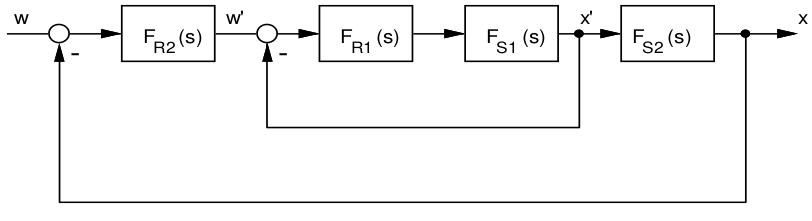
\includegraphics[width=0.9\columnwidth]{Figures/zusammenwirkenMehrererSysteme/Kaskadenregelung.png}

	\begin{mdframed}[style=exercise, frametitle=Führungsgrößenfilter:]
		Falls eine Nullstelle den Regelkreis dominiert (nächster zur Imaginärachse) kommt es zu einem einzelnen Überschwinger. \\
		Zur Vermeidung wird in den Zweig der Führungsgröße ein \(PT_1\)-Filter eingefügt, welches die Nullstelle genau kompensiert.
	\end{mdframed}

	\begin{mdframed}[style=exercise, frametitle=Anti-Windup:]
		Wenn ein Regler mit I-Anteil und eine Begrenzung der Stellgröße vorliegt, kann es zum „Windup“ kommen: I-Anteil wird immer größer, da die Stellgröße begrenzt ist. Dies führt zu Überschwingen. \\
		Anti-Windup: Begrenzung des I-Anteils, damit er nicht über die Stellgrößenbegrenzung hinauswächst.
	\end{mdframed}
